\chapter{Method}
\label{chap:method}

% \thispagestyle{fancy}
% FIXME -- change from cross model to vae-gan

This chapter presents the details and the motivation behind the design choice of the neural network such as the architecture, loss function, optimizers along with the training and evaluation procedure.

\section{Architecture}
To predict root-relative 3D pose solely using 2D poses, a hybrid network using \ac{vae} and \ac{gan} as discussed in \ref{subsec:vaeganhybrid} is employed. In contrast to the \ac{vae}-\ac{gan} hybrid introduced in \cite{autoencoding_beyond_pixels} where only the decoder acts as the generator, both the encoder and the decoder are considered as the generator in the proposed approach. In other words the encoder is also updated to maximize the probability of fooling the discriminator. The overall architecture is illustrated in the Fig \ref{fig:method_arch}. The following is the design and working of each of the components of the proposed \ac{vae}-{gan}.

\subsection{Encoder}

Adding to the explanation of \ac{vae} in \ref{subsec:vae}, the role of the encoder is to take a 2D pose as input and estimate its latent representation in the form of mean and standard deviation. The encoder consists of an upsampling layer that scales the $2 \cdot j$ dimensional input to match the number of hidden neurons of the encoding module. Where $j$ is the number of joints, here 16. The encoding module is made of $n$ residual block composed of 2 \ac{fc} layers following the related works, to allow comparison. Where $n$ is usually 1 or 2, 2 is chosen for most of the experiments. The enoding block is followed by 2 \ac{fc} layers that downsample the hidden representation to match the latent space dimension. The output of the two downsampling layers represents the mean and standard deviation of the embedding in the latent space. However in practice, the encoder is designed to predict log-variance instead of the standard deviation to have a better distribution of values and gradient. 

\subsection{Decoder}

The decoder takes the 2D pose embedding $z$ derived from the mean and log-variance predicted by the encoder and estimates the corresponding 3D pose. The reparametrization trick is used to make the process differentiable and induce variance. This is done by scaling the standard deviation obtained from the log-variance with a random sample from a unit gaussian distribution $\mathcal{N}(0,1)$. The sum of the scaled standard deviation and the mean gives the sample $z$. Similar to the encoder, the decoder consists of an upsampling layer that scales the sample $z$ of the latent space dimensions to match the number of hidden neurons in the decoding module. The decoding module is identical to the encoding module and consists of $n$ residual blocks composed of 2 \ac{fc} layers. This decoding module is followed by a \ac{fc} layer to downsample the neurons to predict 3D pose of dimension $3 \cdot j$. 

Since the 3D is projected to 2D to form the reconstruction loss, the distance between the head and the pelvis joint should approximately be of unit length as explained in \ref{processing}. To achieve this, a Tanh activation function is used to obtain the predicted 3D pose (all joints) in the range [-1, 1]. However, the length of the lower half of the pose can be longer that the upper half and usually is the case. Hence the predicted 3D pose is scaled by a factor of 1.3, the ratio of the mean length of the upper and lower halves, to enforce the length of the upper half to ~1 unit and get the best 2D re-projection.

\begin{figure}[h]
    \centering
    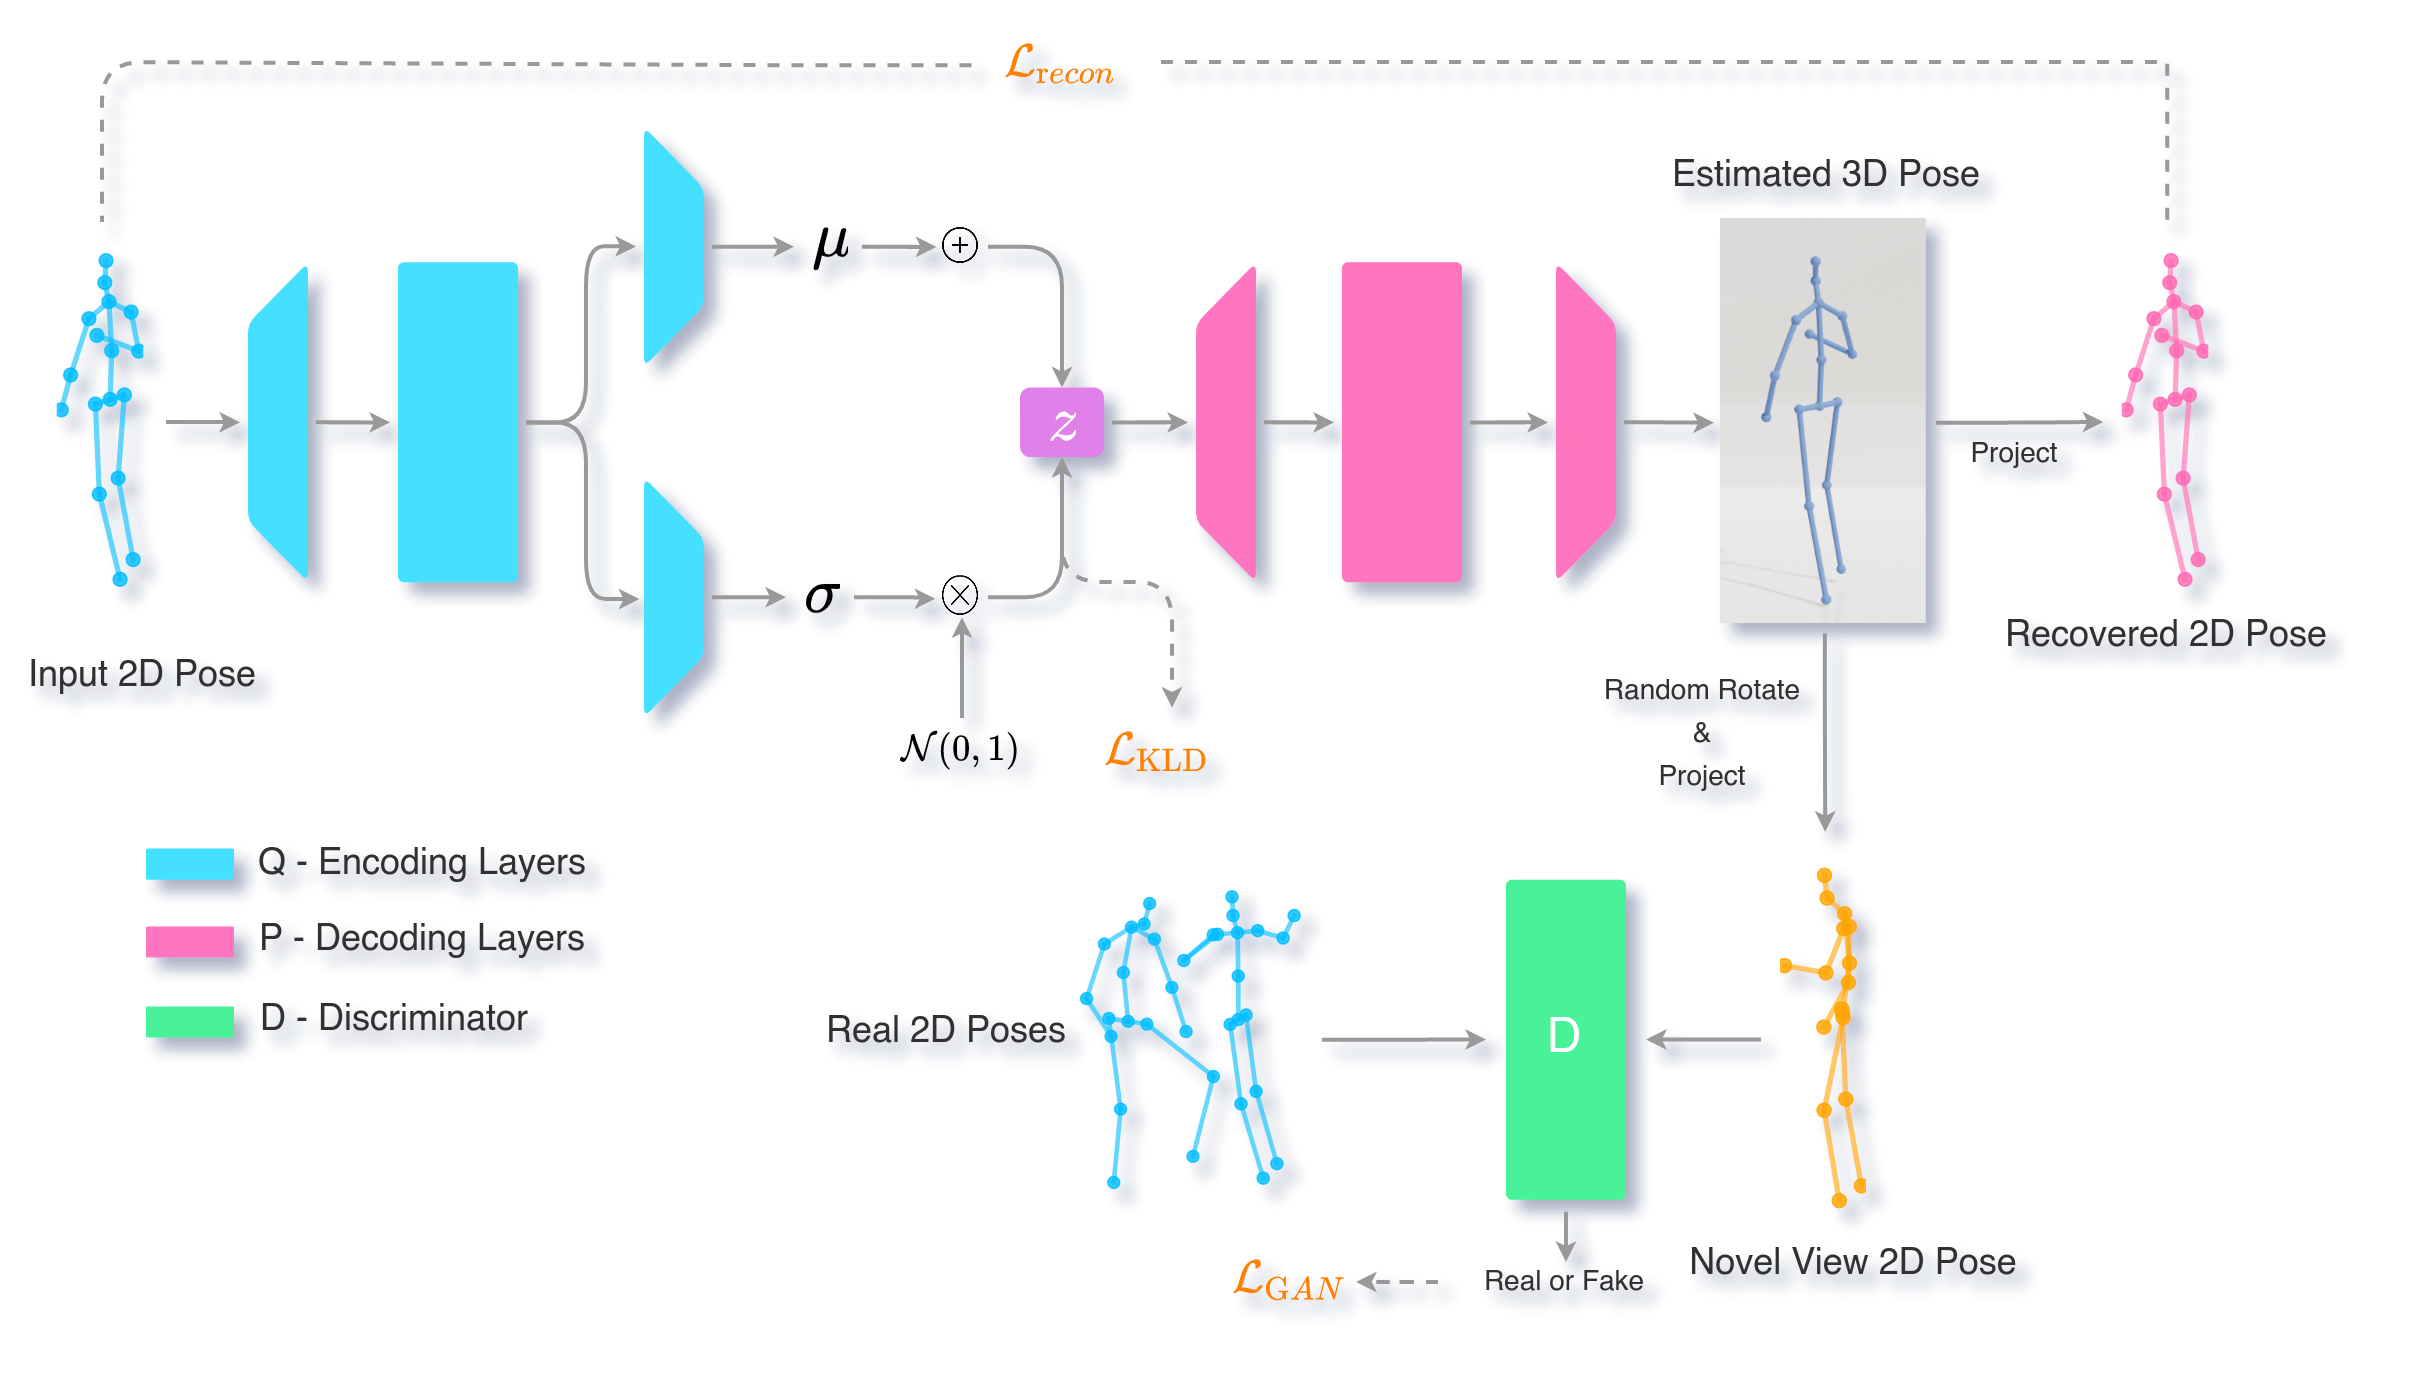
\includegraphics[width=\textwidth]{figures/arch/method_arch.png}
    \caption{Illustration of the neural architecture of the proposed method. The network components in blue, encode the 2D pose to a latent representation in terms of mean $\mu$ and standard deviation $\sigma$ of the distribution. While the components in pink, sample $z$ from this latent space and decode the corresponding 3D pose. The 3D pose is projected directly to 2D space for a constrained optimization using input 2D pose in the camera view and randomly rotated and projected for unconstrained optimization using the discriminator $D$ in a novel angle. The data that contributes to the loss function in orange, are mapped with a dotted line.  
    }
    \label{fig:method_arch}
\end{figure}




Following the best practices from \cite{soumith2017wasserstein}, the decoder (and the encoder) which acts as the generator for the \ac{gan} is made to output 3D poses with values from [-1,1]. 
%FIXME blunder in the implementation?
All the layers use \ac{relu} activation unless specified otherwise. The decoder mimics the encoder with an upsampling layer, a decoding module, and a downsampling layer to output 3D pose of dimension .

% -1 to 1 ...scale to meet the head as 1. 
% initalization activation optimier
% at activation mention that the scaling of -1

\subsection{Discriminator}%FIXME -- \subsection{Image \ac{vae}}
The discriminator following the related works also mimics the generator and takes 2D poses as input and predicts binary labels of real or false. The sigmoid activation function is used at the output layer of the discriminator.

\subsection{More on Activation functions}
beta scheduling cycling and o to 1 annealing, weighting the loss components

%FIXME
\subsection{Loss Functions}
beta scheduling cycling and o to 1 annealing, weighting the loss components

\subsection{Optimizers Functions}
beta scheduling cycling and o to 1 annealing, weighting the loss components


\section{Training Scheme}
The training scheme is similar to the standard \ac{vae} and \ac{vae}-\ac{gan} introduced in \ref{sec:Preliminary}. The discriminator is trained first for a few steps before training the \ac{vae}. First, the \ac{vae} takes the 2D pose as input and predicts the 3D pose. This predicted 3D pose is first reprojected to 2D to train the \ac{vae} and then randomly rotated and reprojected to a novel 2D view. This novel 2D is used as fake samples to train the discriminator. As \ac{vae} learns to improve the reprojected 2D pose, it will eventually be very close to the real samples. Using these as the fake examples will not be very useful as the decoder does the same job. Training the discriminator on a randomly rotated and reprojected 2D novel view would encourage the decoder to generate a pose that not only agrees with the input 2D pose but ensures that the other view of the 3D is also indistinguishable from the variations found in the data by fooling the discriminator. This two-view supervision leads to better 3D pose generations.

% \section{Bag of tricks} % TODO -- add tricks to make it work here or at work? -- it should be here
% \lipsum[1-10] %FIXME

\section{Evaluation Metrics} % FIXME
3D \ac{hpe} and Human3.6M in particular is mainly evaluated by \ac{mpjpe} metric. MPJPE as it abbreviates is the mean of the position estimate for all the joints of a pose. Where per-joint position estimate is nothing but the euclidian distance (usually measured in mm) between the predicted joint to its ground truth.


\begin{figure}[h]
    \centering
    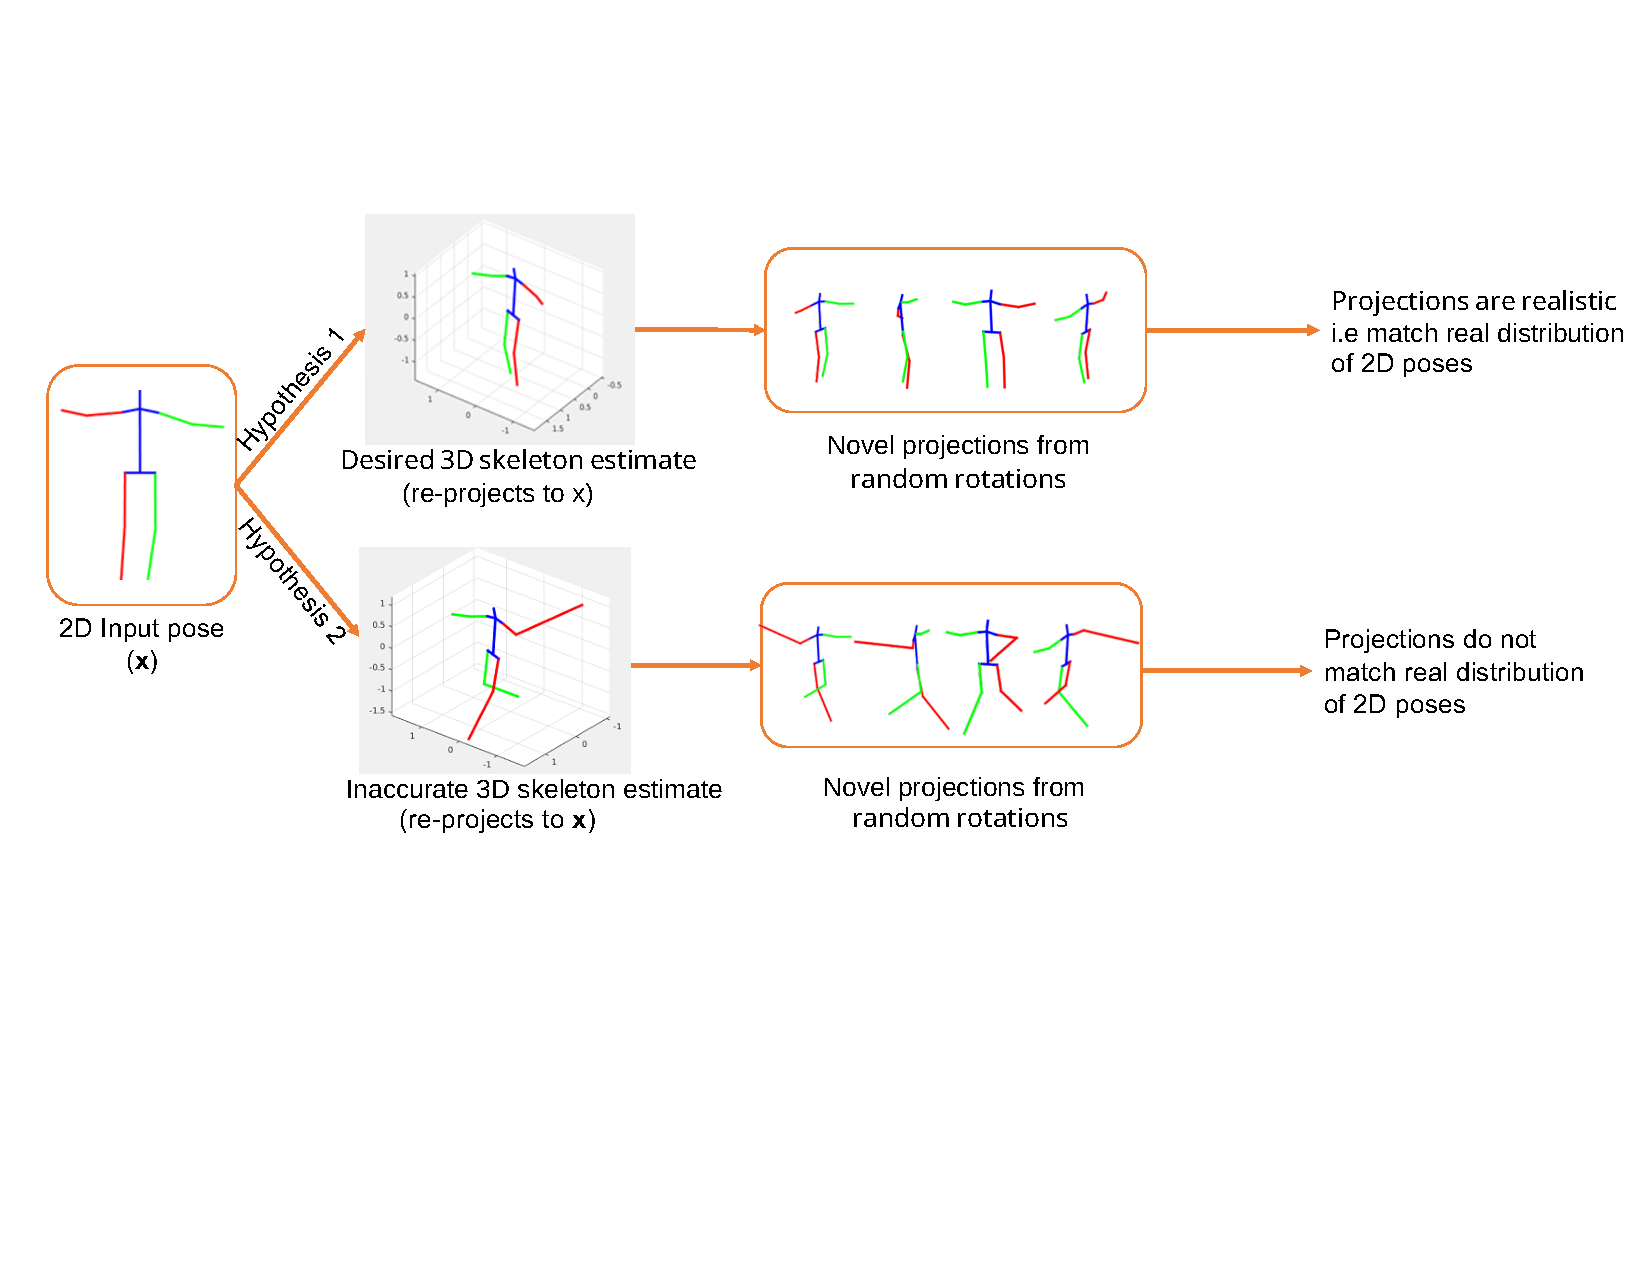
\includegraphics[width=\textwidth]{figures/h36_viz/novel_view_contraint.pdf}
    \caption{Illustration of the architecutre and loss flow in the proposed approach.}
    \label{fig:novel_view_constraint}
\end{figure}

% \section{more details the model prints?} % FIXME
